\documentclass[oneside]{report}
\usepackage{suthesis-ug}
\usepackage{graphicx}
\usepackage{apacite}

\usepackage{array}

% this is for cite by numbers: [3] 
\usepackage[square,sort,compress,numbers]{natbib}
\usepackage[pdftex,colorlinks=true]{hyperref}
\usepackage[bottom]{footmisc}

\usepackage{amssymb}
\usepackage{bbm}
\usepackage{amsmath}
\usepackage{float}


% numbering in references but have an error
\usepackage[natbibapa]{apacite}
\makeatletter
\renewcommand\@biblabel[1]{[#1]}%

\dept{Mathematics and Mechanics}
\begin{document}
\setstretch{1.3}
    \title{Master Thesis\\ Emotion Recognition Using Fusion of Audio and Video Features}
\author{Grigor Keropyan}
\principaladvisor{Vazgen Mikayelyan}
\patitle{Avetik Karagulyan}
\padept{Department of Mathematics and Mechanics}

\coprincipaladvisor{Grigor Keropyan}
\copatitle{s}
\copadept{Statistics}

\beforepreface
\prefacesection{Abstract}
    Emotion Recognition is ability to understand what fillings are others want to transfer. Emotion Recognition is possible to done from a different modalities (e.g. speech, video, text, etc). Understanding others transferred fillings is important for the reasons: in human-human interaction and human-computer interaction. As understanding emotion even is not easy for humans it is a great challenge for computers being able to recognize emotions with a high accuracy. However, with the rapid development of the field of Machine Learning and Deep Learning it seems reasonable to apply this techniques in Emotion Recognition. 
    Existing methods for Emotion Recognition mainly are divided into three parts: feature level fusion, decision level fusion and hybrid fusion (which will be discussed in the following chapters in more detail). First two missing the principle to use the whole content of multi-modality, However, hybrid fusion could reasonably use the existing information in multi-modality and have a chance to outperform existing methods. 
    This work explores multi-modal (Audio and Audio-Video fusion) Emotion Recognition using Deep Learning techniques and the method is based on the hybrid fusion. 

% \prefacesection{Acknowledgements}
%     This is a Master Thesis at YSU 

\afterpreface
\chapter{Introduction}

    Emotions are indivisible part of humans life and play an important role in different types of interactions \cite{af_computing}. In human-human interactions, recognizing others emotion is deciding factors how deeply people understand others. Moreover, in human-computer interactions (HCI) \cite{hci_1, hci_2}, emotions are becoming an vital as the interaction between humans and computer growing rapidly. Taking into account COVID-19 situation, this last year most of the universities have changed their studies from onsite to online and teaching is becoming more challenging. Having a good autonomous emotion recognizer could help improve the current situation by making people's life easier providing some feedback about their emotional state during a conversations and lectures. Also, Emotion Recognition (EM) is promoting to a harmony of HCI \cite{google_survey} (e.g. using a phone which understands the owner emotion and provides corresponding recommendations). 
    
    
    Usually expressing emotion is possible through speech, text, video, etc.  It is an important point to state that emotions can vary from culture to culture and so, in particular models that learned on in English does not mean they perform well also on Spanish. As a consequence it is possible that deciding factors for emotions can be different from language to language. In the literature emotion expression activities are known as modalities. If the model is recognizing emotion based on the only one  activity it is called uni-modal and if it is based on more than one it is called multi-modal. Logically, uni-modal models should not have high accuracy as they have less information (e.g. only facial expression, audio, etc.). In fact, as \cite{google_survey} describes in the introduction for the overall emotion semantic content contributes only by $7\%$, while the semantic content and facial expression contribute $38$ and $55\%$ respectively. On the one hand, facial expression and gestures are important for emotion expression as new born child can only see such things and mainly get impression from these modalities, however, they are not enough for getting a state of the art models. That is why in recent year researchers are using data fusion strategies in order to get high performance as the authors have done in \cite{china_2020}. In data fusion strategies the main point is to extract important features for emotion from a different modalities and using combination of them to recognize emotions.
    
    
    As recently Machine Learning (ML) and Deep Neural Networks (DNN) are growing in a constant high rate and having a good results of them in a variety of fields, it is reasonable to try to ML and DNN in Emotion Recognition. During last two decades a lot of research have been done in the direction \cite{china_2020, stanford_2020, india_2020, slovenia_2014, waterloo_2019, estonia_2018, stuttgart_2021, china_2020_1, india_2014}. Most of mentioned researches using some kind of features from an audio and/or videos and giving these as an input for Machine Learning or Deep Learning models. With the time accuracy of the models are getting higher, however, there is no state of the art work that have been done yet in this field and here a lot of research is needed. As one expects, for the above mentioned methods proper datasets play a key role. As described in \cite{google_survey} already there are some datasets which is reasonable to use for the training of the new models. 
    
    Datasets that are used in this work are described in following chapter in more detailed. One of the problems is the lack of many speakers: as having a few speakers in the existing datasets will not guaranty generalization toward new speakers that the model have not seen. That is why in this work the test data is consists only from the speakers whom the models have not seen during a training time. If the performance of a model is good for this test dataset it is more logical to think that this model generalization error is less than the others which have been tasted only on data which is familiar to the model. This is one of the key difference between this work and the others mention above. 
    
    
    Following are the key developments that have been done during in this work.
    
    \begin{enumerate}
        \item Use hybrid method for modality fusion on the raw data (audio and pictures from video)
        \item Train and test sets separation based on the speakers (this is important as models tend to overfit to speakers and so the generalization error will be high in this cases)
        \item Use mixture of different datasets with augmentation of real world noise in order to provide robustness
    \end{enumerate}



\chapter{Existing Datasets and Methods}

\section{Datasets}

    
    This section is an overview of existing datasets for an audiovisual emotion recognition. As most of the datasets are in English and this work is based on English datasets here is only a description for English datasets. For more general class of datasets refer to \cite{google_survey}. Table 
    \ref{table:datasets} shows the datasets and brief information about them.
    
    
    RAVDESS \cite{RAVDESS} is audiovisual dataset where number of actors are 24 in which 12 females and 12 males. It has only audio for audio emotion recognition. In the Audiovisual part of the dataset consists of speech and song videos. In the song part of the dataset, actors express emotions like they are singing and in the other part is just a causal speech. Each actor speaks two different sentences in eight different emotions (neutral, calm, happy, sad, angry, fearful, disgust, surprised). SAVEE \cite{savee} is audiovisual dataset for four different male actors. Each actor speaks 15 different sentences with seven different emotions (anger, disgust, fear, happiness, sadness, surprise, neutral). IEMOCAP \cite{iemocap} is one of the important  datasets that exist currently in a sense that it contains 12h video recordings with ten different emotion categories (happiness, anger, sadness, frustration, neutral, surprise, fear, disgust, excitement and other). Here, depends on the emotion the dataset can contain very little or very much recording from that part. For instance, other emotion is consists less than one percent and excitement is the most common emotion in the whole dataset. In IEMOCAP ten actors (5 female and 5 male) perform a dyadic (human-to-human) conversations with the above mentioned emotions. eNTERFACE'05 \cite{enterface} 44 actor speak in six different emotions (anger, disgust, fear, happiness, sadness, surprise). Each actor speaks exactly once for each emotion. Here dataset is less than compared to IEMOCAP. SEMANIE \cite{semanie} is 1166 conversations with 150 participants in 27 associated emotional categories. AFEW (Acted Facial Expressions in the Wild) \cite{afew} is a dataset extracted from movies where the intention has been that in each part faces should express some emotion. It contains 1426 sequences of 330 subjects movie parts. The emotions for this dataset are seven (anger, disgust, fear, happiness, neutral, sadness, surprise). 
    
    Here are missing some other datasets which are either not in English or could not been used fro this work. The dataset that have been in this work are from these \ref{table:datasets} datasets and information about them is in the next section. 
    
    \begin{table}[ht!]
    \centering
    \begin{tabular}{ | m{2.3cm} |  m{3cm} | m{2.1cm} | m{6cm} |} 
    \hline
    Dataset & number of speakers & number of samples & emotion info \\ 
    \hline
    RAVDESS \cite{RAVDESS} & 12 female speakers 12 male speakers & 2880 utterance & Eight emotion categories: neutral, calm, happy, sad, angry, fearful, disgust, surprised  \\ 
    \hline
    SAVEE \cite{savee} & 4 male actors & 480 utterance & Seven emotion categories: anger, disgust, fear, happiness, sadness, surprise, neutral \\ 
    \hline
    IEMOCAP \cite{iemocap} & 5 females 5 males & 12h & Ten emotion categories: happiness, anger, sadness, frustration, neutral, surprise, fear, disgust, excitement and other \\
    \hline 
    eNTERFACE ’05 \cite{enterface}  & 8 females 34 males & 1166 video sequences & Six emotion categories: anger, disgust, fear, happiness, sadness, surprise \\
    \hline
    SEMAINE \cite{semanie} & 150 participants & 959 conversations & 27 associated categories \\
    \hline
    AFEW \cite{afew} & 330 subjects & 1426 sequences & Seven emotion categories: anger, disgust, fear, happiness, neutral, sadness, surprise \\
    \hline
    \end{tabular}
    \label{table:datasets}
    \caption{Audiovisual datasets}
    \end{table}


\section{Methods}

    Based on the existing methods for emotion recognition methods are divided into two groups. First one is Machine Learning where the researchers extract some important (important for emotion recognition) features from the audio or video and giving it as an input for Machine Learning algorithms (e.g. Support Vector Machines, XGBoost, Random Forest, etc.) and getting some results on the existing data \cite{india_2020, slovenia_2014, waterloo_2019}. Another group is Deep Learning where the input features can be as raw data as some extracted features from the raw data \cite{muse_2019, stanford_2020, china_2020, estonia_2018, india_2014}. Next is the discussion of features extractions and above mentioned methods in more details. 
    
    
    
\subsection{Features}

    Feature selection is vital for Emotion Recognition as some of them can be  irrelevant for expressing emotions and some of them highly relevant for specific emotion categorization. So, having a right set of features can dramatically improve model accuracy \cite{google_survey}. Following is described Audio and Video features separately. 
    
    \subsubsection{Audio Features}
    
        Here are described some basic features of audio signal.
    
        \begin{itemize}
    
        \item  ZRC: Zero Crossing Rate of audio. It quantifies the rate in which signal changes its sign (from positive to zero to negative or from negative to zero to positive). Formally it is defined as follows: 
        
        \begin{align*}
            zrc = \frac{1}{T - 1} \sum_{t = 1}^{T - 1} \mathbbm{1} (s_{t-1}s_{t})
        \end{align*} 
        
        where \( s \) is a signal of length \( T \) and \( \mathbbm{1} \) is the indicator function. \\
        
        
        \item  RMS: Root Mean Square of audio. It measures the frame energy for signal. RMS is somehow a mean value for digitized signal and can calculated as follows: 
        
        \begin{align*}
            rms = \sqrt{\frac{1}{T} \sum_{t = 0}^{T - 1} s_{t}^2}
        \end{align*}
        
        where \( s \) is a signal of length \( T \). \\
        
        \item HNR: Harmonics to Noise Ratio of audio. It measures the ratio between periodic and non-periodic components of a audio. HNR can be calculated as follows:
        
        \begin{align*}
            hnr = \frac{R_{xx}[T_0]}{R_{xx}[0] - R_{xx}[T_0]}
        \end{align*}
        
        where $T_0$ is assumed periodicity and $R_{xx}$ is the auto-correlation function (ACF) and estimated as,
        
        \begin{align*}
            R_{xx}[l] = \frac{1}{N} \sum_{t = l}^{T - 1} s_{t}s_{t - 1}
        \end{align*}
        
        for the biased version, and as 
        
        \begin{align*}
            R_{xx}[l] = \frac{1}{N-l} \sum_{t = l}^{T - 1} s_{t}s_{t - 1}
        \end{align*}
        
        for the unbiased version. \\
        
        \item  Mel Spectrogram: this is a Mel scale of a Spectrogram which measures the spectrum of the frequency of a audio signal over time.
        The transformation from the Hertz scale to Mel scale is the following:
        \begin{align*}
            m = 1127\log(1 + \frac{f}{100}),
        \end{align*}
        where the $log$ is in natural base. \\
        Spectrogram is computed as Fast Fourier Transform (FFT) of overlaping windows in a audio signal. 
        
        \item  MFCC: Mel-frequency cepstral coefficients. They are the coefficients of the MFC (Mel-frequency cepstrum) which is a short-term power spectrum of a audio, based on linear cosine transform of a log power spectrum on a non-linear mel scale of frequency. MFCC can be calculated as follows:
            \begin{enumerate}
                \item  Fourier transform of a audio signal.
                \item Map the powers of the spectrum obtained above onto the mel scale, using triangular overlapping windows.
                \item Logs of the powers at each of the mel frequencies.
                \item Discrete cosine transform of the list of mel log powers, as if it were a signal.
                \item The MFCC are the amplitudes of the resulting spectrum.
            \end{enumerate}
        
        \item Spectral Centroid: This is a measure to characterize a spectrum. Spectral Centroid indicates where the center of mass of the spectrum is located.
        
        \item Chromagram: This is a the projected spectrum onto 12 bins representing the 12 distinct semitones (or chroma) of the musical octave.
        
        \end{itemize}
           
    \subsubsection{Video Features}
    
    The most relevant features for Emotion Recognition (ER) in a video are body movements and faces expressions. However, the latter one should be more important for ER. The most common approach is to extract faces from the video then using directly the faces or some other important features from the faces. In Figure \ref{fig:ffp} (taken from \cite{google_survey}) is shown 68 facial feature points (FFPs) from five facial regions (eyebrows, eyes, nose, mouth, and facial contours). As different people have different facial animation parameters (FAPs), researchers do further normalization. For each face FAP's expressed by FAP units which is the fraction of key distance in the face. From these points it is possible to extract various types of features which will be the video features. For instance, outer raised eyebrow FAP's is calculated as the distance between 22, 28 and 16, 33 FFP's. Another feature extraction method is to take the whole pictures of faces and force a model to learn emotion form the entire face. 
    
    
    \begin{figure}
    \centering
    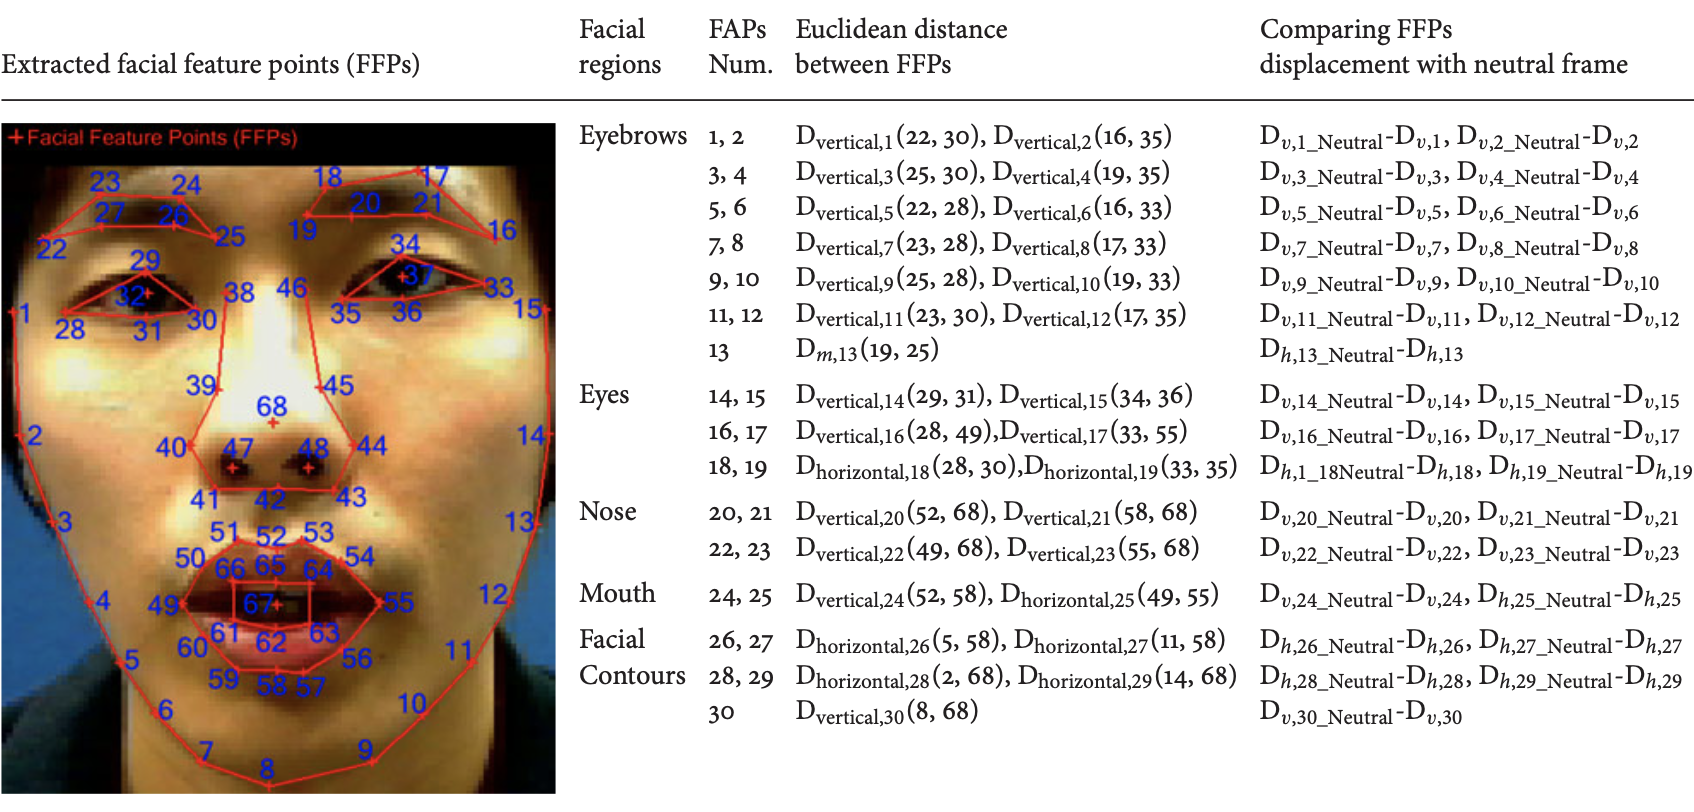
\includegraphics[scale=0.5]{ffp.png}
    \caption{The example of 68 facial feature points extracted using AAM alignment and related facial animation parameters.}
    \label{fig:ffp}
    \end{figure}

\subsection{Bi-modal Approaches}

    For the case of uni-modal Emotion Recognition there is only one type of features (only audio, only video, only text, etc.) which will be the input of any model. However, in multi-modal cases careful fusion of data is important in order to get better accuracy. Based on the existing methods it is possible to divide these approaches into three groups: feature level fusion, decision level fusion and hybrid fusion \cite{feature_fusion1, feature_fusion2, feature_fusion3, china_2020, stanford_2020, india_2020, slovenia_2014, waterloo_2019, estonia_2018, stuttgart_2021, china_2020_1, india_2014}. Each of them are described in the following:
    
    \begin{enumerate}
        \item Feature level fusion: Here fusion strategy is that features are merged in a early level of the model Figure \ref{fig:flf} and then based on that model start to learn how to recognize emotions \cite{feature_fusion1, feature_fusion2, feature_fusion3}. Here are some problems as features are from different modalities can be incompatible for a model and at the end model decision could be based only on one modality which will not improve the accuracy of the model.
        
        \begin{figure}[H]
        \centering
        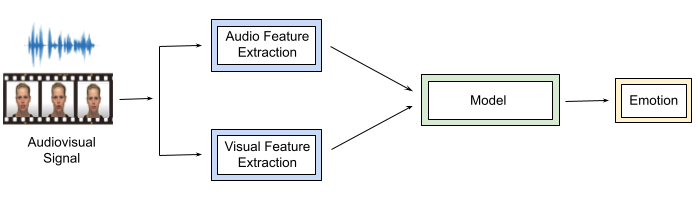
\includegraphics[scale=0.6]{flf.png}
        \caption{Feature level fusion.}
        \label{fig:flf}
        \end{figure}
        
        \item Decision level fusion: Here fusion strategy is totally separates features and actually whole model is based on two sub-models Figure \ref{fig:dlf} and fusion is hold at the last stage \cite{india_2020, slovenia_2014}. Having two networks for two different modalities each of them can predict emotions with some accuracy. Combining their predictions can improve the accuracy in some level. Image on of them predicts happy class more precisely and the other sad class. Final result can be taken happy if the first model predicts happy and sad if the latter predicts sad which defiantly will improve existing models. However, there are other decision-level fusions as some combination of two predictions, majority vote, etc. In these approaches actually models learn separately and the best is that when taking the best result from each of them, which means they do not use the whole existing content of the data. 
        
        
        \begin{figure}[H]
        \centering
        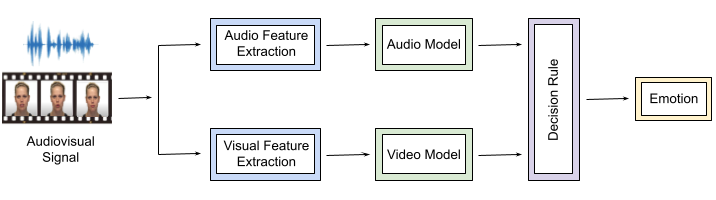
\includegraphics[scale=0.6]{dlf.png}
        \caption{Decision level fusion.}
        \label{fig:dlf}
        \end{figure}
        
        \item Hybrid fusion: As it is clear form the previous approaches there is trade-off around the fusion of the data and the hybrid method is the combination of them \cite{china_2020, stanford_2020, waterloo_2019, estonia_2018, stuttgart_2021, china_2020_1, india_2014}. The idea is that at the beginning two sub models extract important features from different modalities and then combine them at some stage then merged model learn based on that Figure \ref{fig:hf}. This method could combine best sides of two previously described ones as in the first part models can learn features from videos and audio which will be appropriate to combine and last part of the model will learn based on these features.  
        
        \begin{figure}[H]
        \centering
        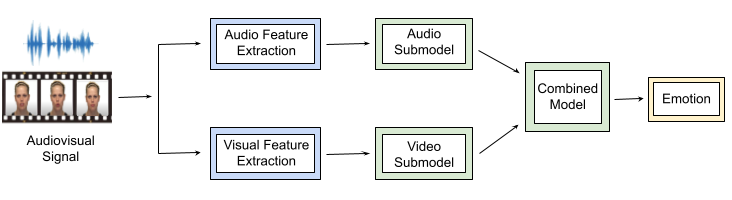
\includegraphics[scale=0.6]{hf.png}
        \caption{Hybrid fusion.}
        \label{fig:hf}
        \end{figure}
        
    \end{enumerate}

    \subsubsection{some models}
    Chennoor et. al., \cite{india_2020} used Machine Learning methods (SVM, KNN) to predict emotions from audiovisual signals. Their methods uses decision level fusion in the following way: if predicted emotions for the audio and video models differ more than fixed threshold then video emotion is the final prediction, otherwise final prediction is audio model emotion. 
    
    In the \cite{stanford_2020} the authors used Deep Neural Networks to predict four and three kinds of emotions, that are: happy, angry, sad, neutral in the IEMOCAP \cite{iemocap} dataset. They used Spectrograms as feature from audio and 20 extracted faces from a video (each video is 3 seconds long or less). Model is a hybrid type consists of CNN for pictures, CNN+RNN for audio and fully connected for last stage. 
    
    Zhou et. al., \cite{china_2020} used AlexNet and ResNet for extracting features for aduio log-mel spectrogram and video pictures coresspondingly and then used Hybrid approach. The use of AlexNet and ResNet can be dramatically improve the accuracy of a model as these networks can extract important features from the raw (pictures, Spectrograms) data, however, it has a additional layer inside model and clearly will increase prediction time. 

\chapter{Proposed Method}

    Based on the existing methods the one which has the power to exploit the whole content of the multi-modal data is hybrid approach. In this case the method may be able to use the proper mixture of the semi-learned features and improve the emotion recognition accuracy. In order to understand whether or not the proposed methods have been able to exploit multi-modal features, the results are compared with the baseline results \cite{stanford_2020} and also best audio model accuracy is compared with the best video model accuracy. In the latter case if the video model accuracy is better than audio model accuracy it means hybrid model have been able to use features from both modalities effectively and if the accuracy is better than the baseline it means the method is also effective. 
    
    \subsubsection{Datasets}
    
    Datasets are chosen in way that they will be in English, contain as many speakers as possible and have been able to capture the real world examples. Being English is important as for the different languages features could vary and it could affect on the result dramatically and existing datasets are mainly in English. As explored in this work generalization of the emotion recognition algorithm is much more difficult in the case of new speakers. So, having more speaker is helpful to overcome this problem. The latter case is important as for the application in the world the algorithm should be able to recognize emotions from the real world cases. Based the above mentioned criteria the following datasets are chosen: Imeocap \cite{iemocap}, eNTERFACE'05 \cite{enterface} and RAVDESS \cite{RAVDESS}. Each video is divided into 3 seconds long sub-videos. Each sub-video is one input for the model. As the existing labels of the datasets are dramatically unbalanced only four labels (happy, angry, sad, neutral) have been chosen. They are the same labels as in \cite{stanford_2020} paper. At the end the whole dataset is about 12h long. For the sake of good generalization train and validation is divided by speakers. Speaker who are appearing in validation set does not appear in the train set at all. Around 20 percent of the whole dataset separated for the validation set. For the purpose of robustness of the models real world noise is mixed with the dataset. After this data augmentation dataset is increased four times which is also one of the reasons that the models could have been able to overcome the problem of overfitting.
    
        
    
        \begin{figure}[H]
        \centering
        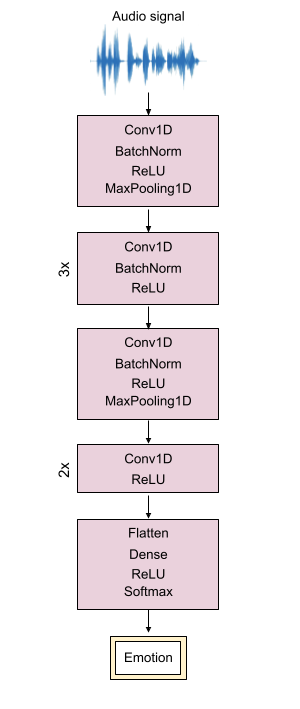
\includegraphics[scale=0.6]{Audio.png}
        \caption{Audio model.}
        \label{fig:audio}
        \end{figure}
    
    \subsubsection{Features}
    In the case of audio, ZRC, Chromogram, MFCC, RMS and Mel Spectrogram have been chosen. Most of the features is posible to get from Spectrogram, however, it is a raw feature and for the models it is additional work to extract important features from Spectrogram. So, providing other features directly could potentially improve the model. At the end each audio feature is (160, 1) array. 
    
    In the case of video, from each video 20 images are taken and from each image only the faces are extracted using Dlib toolbox \footnote{ http://dlib.net/}.
    At the end for each video extracted feature is (50, 50, 20) image. The idea is to choose only faces from the whole image is that visual emotions are mostly expressing by faces and also part of the datasets missing the whole image of the person. 
    
    \subsubsection{Models}
    Throughout the work CNN, Lstm and their mixed networks have been explored. 
    
    For the audio case Figure \ref{fig:audio} one of the CNN models that have been tried. 2x and 3x on the left of the blocks mean that there is 2 and 3 consecutive repetition form the same block respectively. Using a BatchNormalization used to overcome the overfitting problem partially. As in the case of new speaker learned model could not predict emotion in a high accuracy. MaxPooling layers help to reduce the number of weights and models become simpler. At the end of 8th block output have flattened and one dense layer added and then Softmax activation. Lstm network also tried for the only audio case, where the first layer is Lstm then few layers dense and ReLU blocks with Batchnormalization. Also networks with more weights have been tried which tend to overfit and could not genrealize well. 
    
    For the video case CNN-CNN and Lstm-CNN networks have been tried. Until their concatenation audio and video parts learn separately and in some point they concatenated and then some block after it. Figure \ref{fig:video} shows a CNN-CNN model where the audio part is the same as only previously described audio network without Softmax replaced by ReLU. The video part of the network uses Conv2D layers with ReLU and Batchnormalization and some of them MaxPooling. At the end of 5th block Dropout is used in order to prevent form overfiting. After concatenation two layers was used for the hybrid level fusion and at the end Softmax activation. 
        
        \begin{figure}[H]
        \centering
        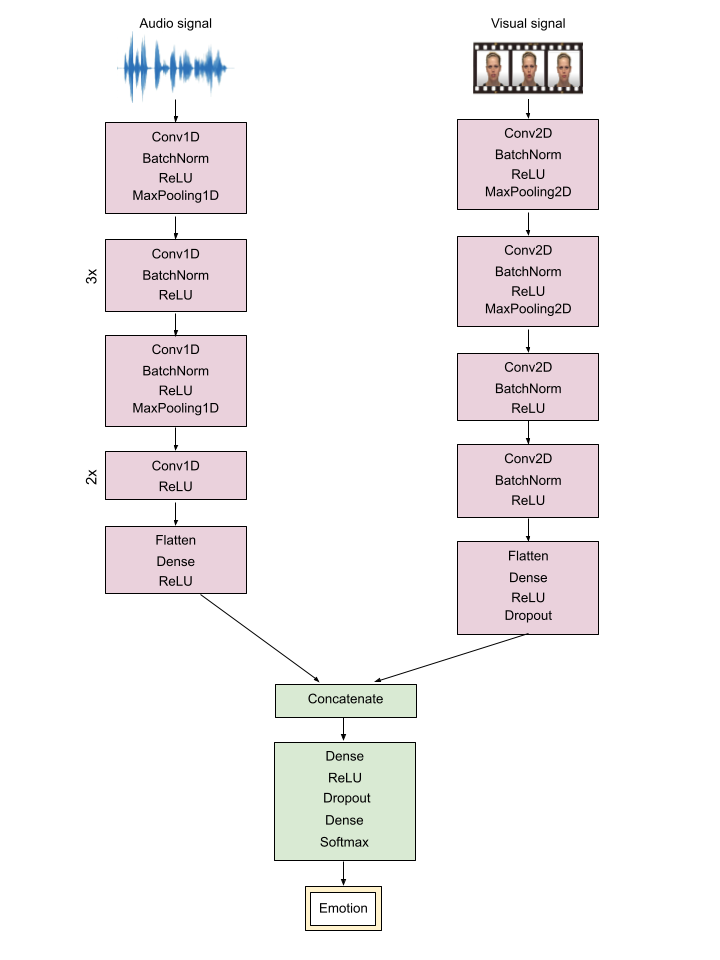
\includegraphics[scale=0.6]{Video.png}
        \caption{Audio model.}
        \label{fig:video}
        \end{figure}

    

\chapter{Experiments and Results}

    Models have been trained using Adam, RMSProp and SGD optimization algorithms with different learning rates (1e-3, 1e-4, 1e-5). The result for the RMSProp and SGD is significantly worse compared to Adam. The best Audio model outperformed \cite{stanford_2020} best video model slightly having more than 54\% accuracy Table \ref{speaker}. Important thing here is that the result is on the unseen speakers. In the case of random split of data models accuracy is more than 87\% Table \ref{random} and shows that described approach is much more powerful than existing ones. 
    
    Video models show better performance than audio models, however, depends on the model they have tendency to overfitting. Best Video model is CNN-CNN model more than 57\% accuracy Table \ref{random}. The accuracy plot of the model is showed in the Figure \ref{fig:accuracy}. \\
    
    \begin{table}[!htb]
    % \caption{Global caption}
    \begin{minipage}{.5\linewidth}
      
      \centering
        \begin{tabular}{ |p{3cm}||p{2cm}|p{2cm}|p{2cm}|  }
         \hline
        models & Accuracy  \\
        \hline
        Baseline & 54    \\
        \hline
        Audio model & 54   \\
        Video model & \textbf{57.7}  \\
        
        \hline
        \end{tabular}
        \caption{Results on speaker split.}
        \label{speaker}
    \end{minipage}%
    \begin{minipage}{.5\linewidth}
      \centering
        
        \begin{tabular}{ |p{3cm}||p{2cm}|p{2cm}|p{2cm}|  }
    \hline
    models & Accuracy random.s. & Accuracy speaker s. \\
    \hline
    Baseline & 54    & - \\
    Lightgbm Audio & \textbf{87.7}   & \textbf{57.6}  \\
    \hline
    \end{tabular}
    \caption{Results on random split.}
    \label{random}
    \end{minipage} 
    \end{table}
        
        \begin{figure}[H]
        \centering
        \begin{minipage}{.5\textwidth}
        \centering
        % \includegraphics[width=.4\linewidth]{image1}
        \includegraphics[scale=0.6]{accuracy.png}
        \caption{Video model accuracy.}
        \label{fig:accuracy}
        \end{minipage}%
        \begin{minipage}{.5\textwidth}
        \centering
        % \includegraphics[width=.4\linewidth]{image1}
        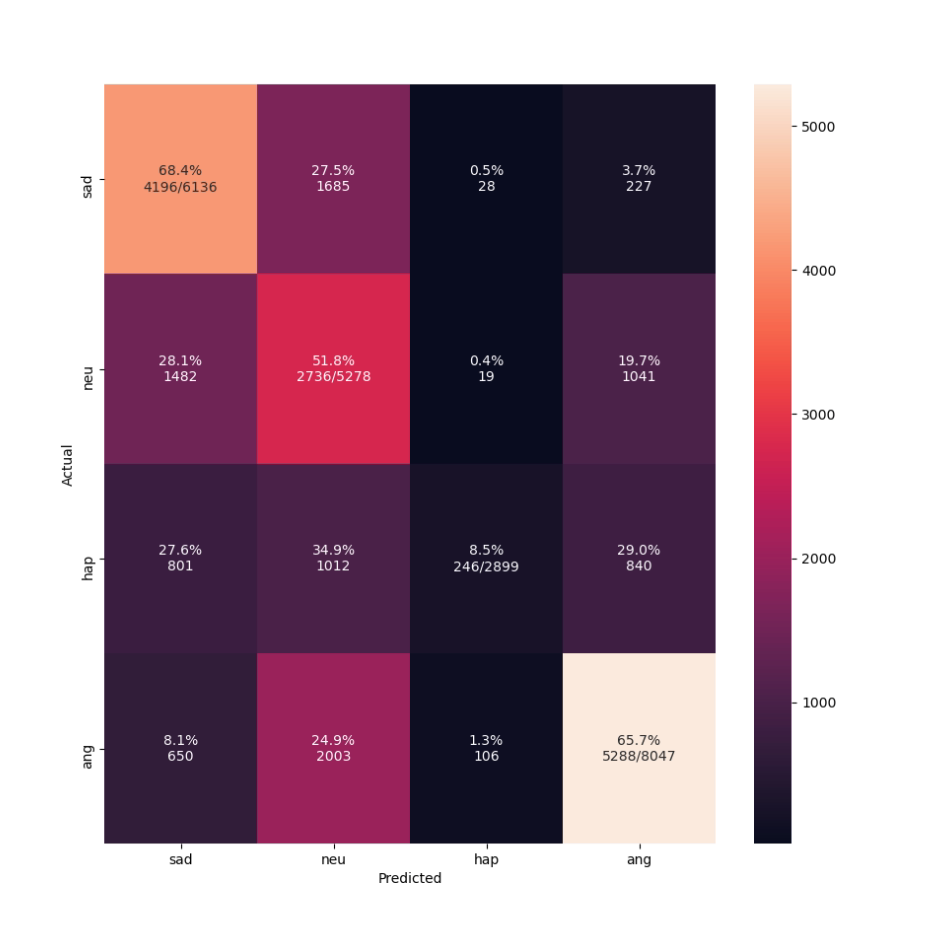
\includegraphics[scale=0.6]{cm.png}
        \caption{Confusion matrix.}
        \label{fig:cm}
        \end{minipage}
        \end{figure}

    
    All the models have trained maximum 100 epochs. In the cases when the train and validation accuracies differ more than 20 percent model traning have been stopped for the sake of not overfitting. The codes are available in GitHub. \footnote{\url{https://github.com/grigor97/multimodal_emotion_recognition}}
    

\chapter{Conclusion}
    In this work new approach have been explored for emotion recognition. Existing methods mainly use the random split of the datasets and they are open to overfiting for the speakers and cannot generalize well. In the proposed method validation dataset is split by speakers and also compared with the random split of the dataset and experimentally showed that the latter one is much more easier to get high accuracy. Based on the experiments it turned out that using a hybrid level fusion help to use the existing content of the multiple modalities effectively by improving model accuracy. Moreover, using fusion of few datasets and similar to real world scenarios help to improve model performance and give an opportunity to use these kind of model in a real world applications. This work has been carried out in a short period of time for the master thesis and having more time would enable to explore existing methods and their performance in a better way. Moreover, being able to effectively use another modality (e.g., text) is promising research area in order to get state-of-the-art models.


% \appendix
% \chapter{True Facts}

% \begin{enumerate}
%     \item we are good!
% \end{enumerate}

\renewcommand{\bibname}{Bibliography}
\bibliographystyle{apacite}
\bibliography{thesiscite}
\end{document}
